%% Handout
%\documentclass[handout,compress,dvipsnames]{beamer} % only complete slides, no "animation"
%\setbeameroption{hide notes} % Only slides

%% Presentation
\documentclass[dvipsnames]{beamer} % complete slides with "animation"
\setbeameroption{show notes}\setbeameroption{show notes on second screen=right} % Slides and notes

\usepackage{pdfpages}
\usepackage{fix-cm}

% adjust note page
\setbeamertemplate{note page}{%
    \pagecolor{yellow!5}
    \vfill
    \begin{minipage}[c][\textheight][t]{\textwidth}
        {\usebeamerfont{frametitle}\usebeamercolor[fg]{frametitle}\insertframetitle\par}
        \insertnote
    \end{minipage}
}

% Theme and coloring
\usetheme{Warsaw}
\colorlet{darkbg}{MidnightBlue}
\colorlet{lightbg}{Cyan!20}
\colorlet{slidebg}{Cyan!5}
\setbeamertemplate{frametitle}[default]
\setbeamercolor{frametitle}{fg=white,bg=darkbg}
\setbeamercolor{framesubtitle}{fg=lightgray}
\setbeamercolor{block title}{fg=white,bg=darkbg}
\setbeamercolor{block body}{bg=lightbg}
\setbeamertemplate{itemize item}[default]
\setbeamercolor{itemize item}{fg=black}
\setbeamertemplate{enumerate item}[default]
\setbeamercolor{enumerate item}{fg=black}
\setbeamercolor{title}{fg=white,bg=darkbg}
\setbeamercolor{background canvas}{bg=slidebg}


%% remove some stuff
\setbeamertemplate{navigation symbols}{}
\setbeamertemplate{footline}{}
\setbeamertemplate{headline}{}
\let\dohead\relax % remove toc header

% Packages
\usepackage{enumerate}
\usepackage{array}
\usepackage{eqnarray}
\usepackage{longtable}
\usepackage{bookmark}
\usepackage{caption}
\usepackage{multido}

% define title with section and subsection
\newcommand{\makeFrameTitle}{
    \setbox0=\hbox{\subsecname\unskip}\ifdim\wd0=0pt
        \frametitle{\secname}
    \else
        \frametitle{\secname}
        \framesubtitle{\subsecname}
    \fi
}

%%% Citation %%%
\usepackage[backend=biber,%
    style=ieee,
]{biblatex}
\addbibresource{bibliography.bib}
\renewcommand*{\bibfont}{\fontsize{8}{8}\selectfont}

% Custom Commands
\newcommand{\slide}[1]{\frame{\makeFrameTitle #1}}
\newcommand{\animationSlide}[1]{\frame<handout:0>{\makeFrameTitle #1}}
\newcommand{\notes}[1]{\note{\begin{itemize}#1\end{itemize}}}
\newcommand{\arrow}{\textrightarrow~}
\newcommand{\defblock}[1]{\begin{block}{Explanation} #1 \end{block}}
\newcommand{\timenote}[1]{\item \textbf{time: #1}}
\mode<handout>{\renewcommand{\timenote}[1]{}}
\newcommand{\hint}[1]{\item \textit{#1}}
\mode<handout>{\renewcommand{\hint}[1]{}}



%Titelseite
\title[]{Latex Beamer Template}
\author{Manuel Philipp}
\institute{Heidelberg University}

%%%%%%%%%%%%%%%%%%
% Begin Document %
%%%%%%%%%%%%%%%%%%
\begin{document}
\begin{center}
    % Titelfolie
    \frame{\titlepage}

    % Outline
    \begin{frame}{Outline}
        % enumeration with items appearing one at a time when not in handout mode
        \begin{enumerate}[<+->]
            \item Section one
            \item Section two
            \item Section three
        \end{enumerate}
    \end{frame}

    %%%%%%%%%%%%%%%%%%%%%%%%%%%%%%%%%%%%%%%%%%%%%
    % Section one
    %%%%%%%%%%%%%%%%%%%%%%%%%%%%%%%%%%%%%%%%%%%%%
    \section {Section one}
    \slide{
        \defblock{
            This is the first section
        }

        \begin{figure}
            \centering
            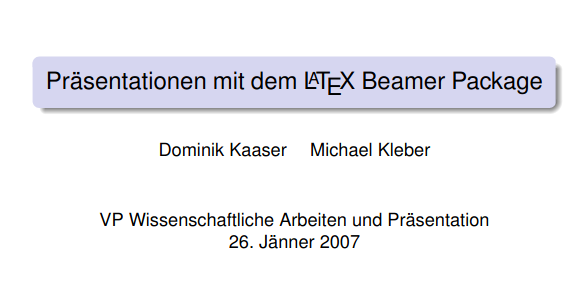
\includegraphics[width=0.45\textwidth]{figures/screenshot.png}
            \caption*{Example Screenshot taken from \cite{kaaser2007latex}}
        \end{figure}

        % Notes
        \notes{
            \item notes for the first section
            \item this includes an image
            % note for expected time at this point. Hidden in Handout mode
            \timenote{1:25}
        }
    }

    \section{Section two}
    \subsection{Pause command}
    \slide {
        \begin{block}{Usage}
            The pause command causes a slide to be split into multiple slides with the each slide only showing stuff before the next pause.
        \end{block}

        \begin{columns}[c]
            \pause
            \begin{column}{0.5\textwidth}
                \begin{figure}
                    \centering
                    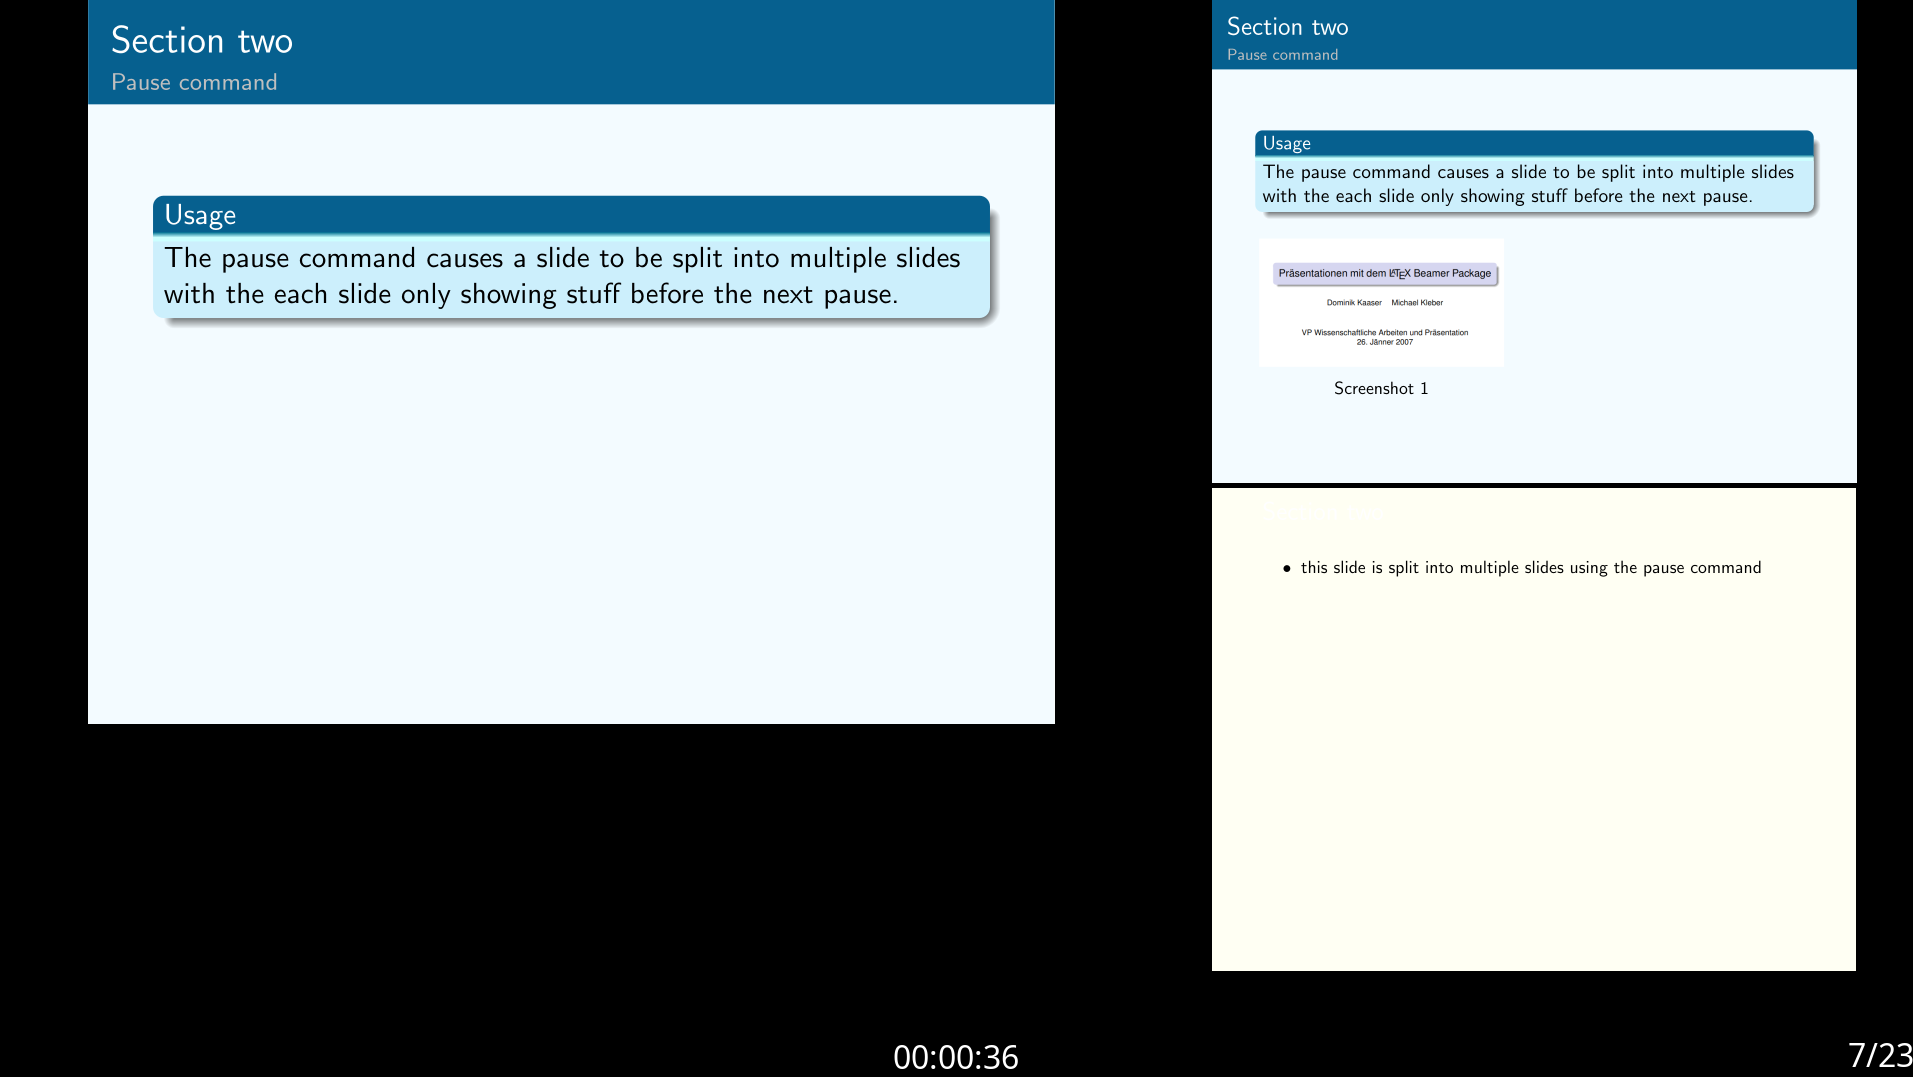
\includegraphics[width=0.9\textwidth]{figures/present.png}
                    \caption*{Presenter Screen}
                \end{figure}
            \end{column}
            \pause
            \begin{column}{0.5\textwidth}
                \begin{figure}
                    \centering
                    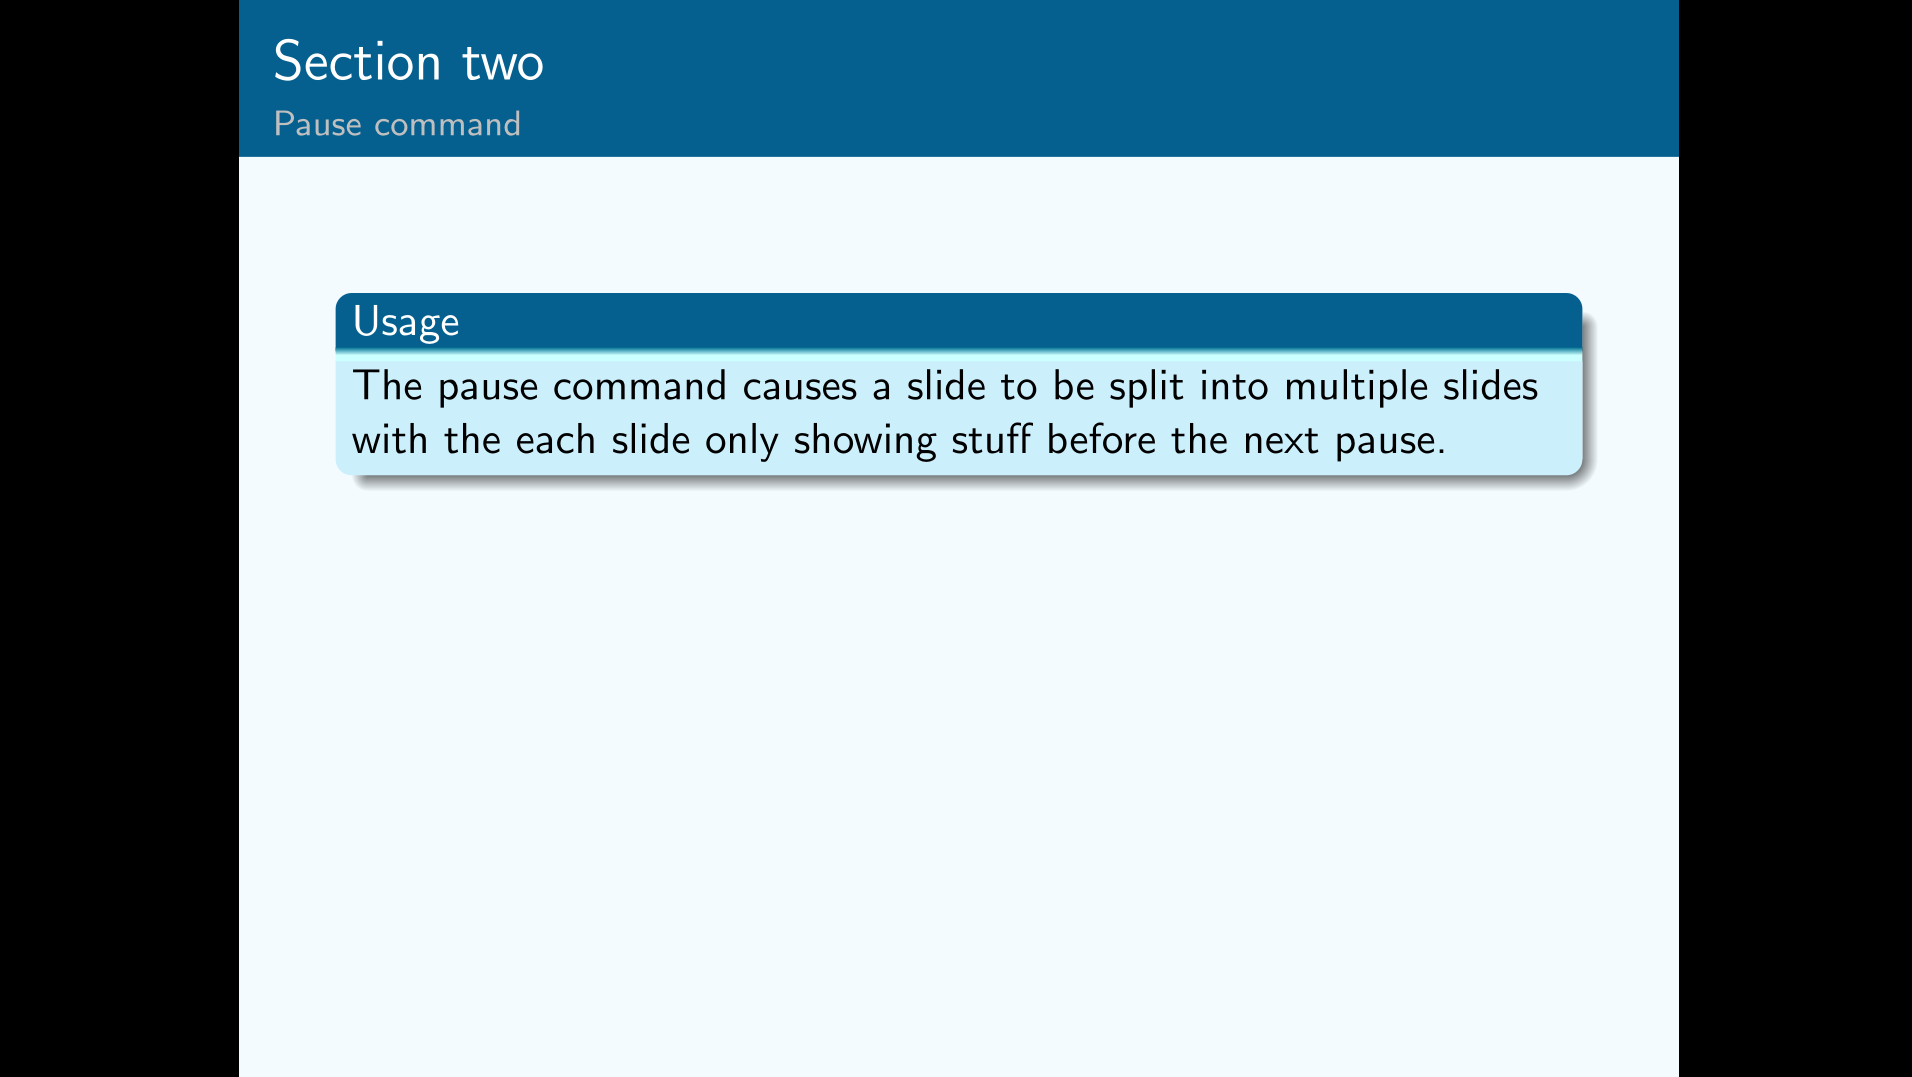
\includegraphics[width=0.9\textwidth]{figures/beamer.png}
                    \caption*{Beamer}
                \end{figure}
            \end{column}
        \end{columns}

        \notes{
            \item this slide is split into multiple slides using the pause command
        }
    }

    \subsection{Animation Slide}
    % animationSlide is a slide hidden in handout mode
    % can be used for "animation" like building up an image
    \animationSlide{
        
\includegraphics[height=\textheight]{figures/animation_1.png}
    }
    \animationSlide{
        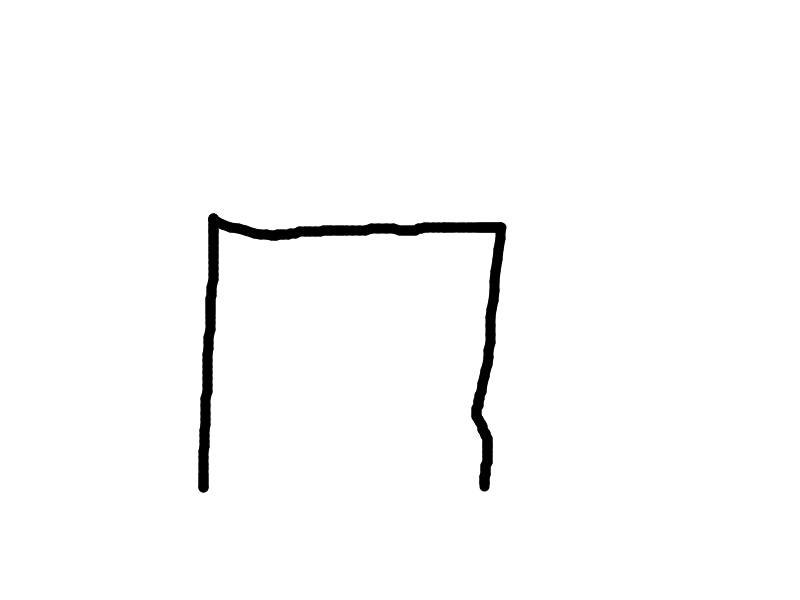
\includegraphics[height=\textheight]{figures/animation_3.png}
    }
    \animationSlide{
        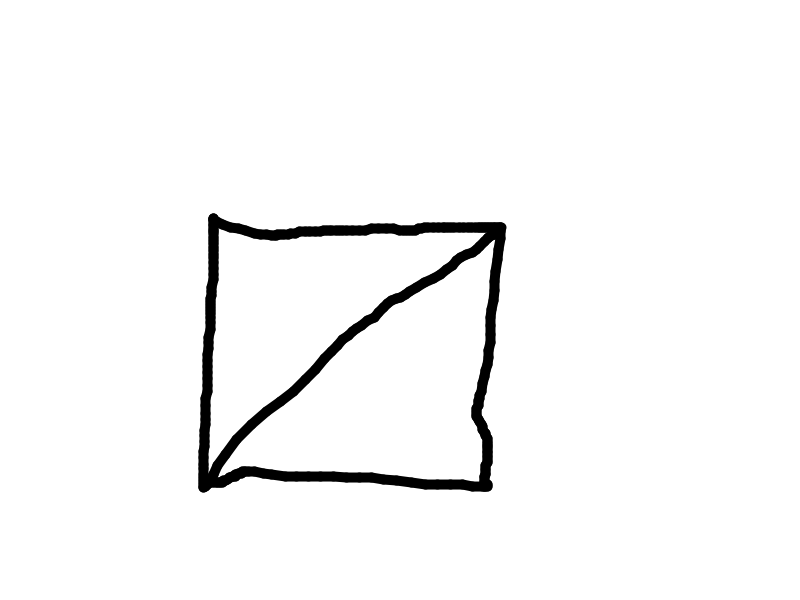
\includegraphics[height=\textheight]{figures/animation_5.png}
    }
    % the last normal slide is always shown
    \slide{
        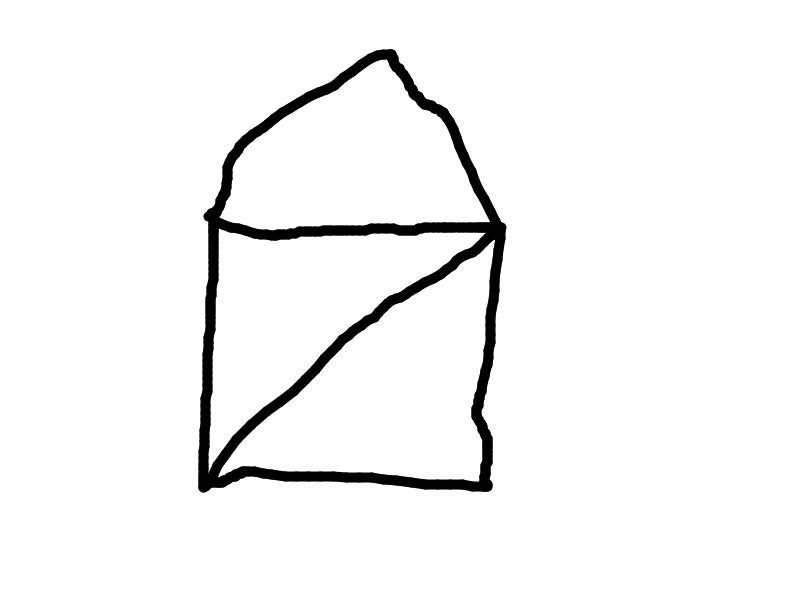
\includegraphics[height=\textheight]{figures/animation_7.png}
    }

    \subsection{Better Animation}
    \slide{
        For Animations with numbered images the multido package can be used.
        %\multido{<var>=<start>+<inc>}{<times}{<stuff>}
        \multido{\i=1+1}{8}{%
            \only<\i>{%
                \includegraphics[height=0.8\textheight]{figures/animation_\i.png}
            }
        }
    }

    % reset section to avoid Heading on slide
    \section{}
    \subsection{}
    \slide{
        \huge{Discussion}
    }
\end{center}

%%%%%%%%%%%%%%%%%%%%%%%%%%%%%%%%%%%%%%%%%%%%%
% References
%%%%%%%%%%%%%%%%%%%%%%%%%%%%%%%%%%%%%%%%%%%%%
\frame[allowframebreaks]{
    \frametitle{References}
    \tiny{\printbibliography}
}


\end{document}

